\section{Experiments}
\label{sec:experiments}

\subsection{Experimental Settings}
\label{subsec:experimental_settings}

\subsubsection{Datasets}
We evaluate our proposed framework on three real-world benchmark datasets derived from the Amazon Review Data (2023 version): Amazon Beauty, Amazon Sports, and Amazon Toys. These datasets vary significantly in domain, scale, and sparsity, providing a comprehensive testbed for evaluating recommendation performance across different scenarios.

Beauty: A dataset with relatively dense interactions, serving as a standard testbed for full-population evaluation.

Sports \& Toys: Large-scale datasets characterized by sparse interactions and long-tail distributions. These allow us to assess the model's capability in handling massive item spaces and extracting signals from sparse behaviors.

To ensure data quality, we convert explicit ratings $\geq 4.0$ into positive implicit feedback, while ratings $< 4.0$ are retained as explicit hard negatives for contrastive learning. We apply a recursive 3-core filtering for both users and items. The statistics of the processed datasets are summarized in Table~\ref{tab:dataset_stats}.

\begin{table}[htbp]
\centering
\caption{Statistics of the processed datasets}
\label{tab:dataset_stats}
\begin{tabular}{lrrr}
\toprule
Dataset & Users & Items & Interactions \\
\midrule
Beauty & 631986 & 115709 & 701528 \\
Sports & 6703391 & 957764 & 12980837 \\
Toys & 4204994 & 624792 & 8201231 \\
\bottomrule
\end{tabular}
\end{table}

\subsubsection{Evaluation Protocols}
We adopt the All-Item Full Ranking protocol. For each test user, the ground-truth item is ranked against all other non-interacted items in the dataset.

\begin{itemize}
    \item \textbf{Metrics}: We report Recall@K and NDCG@K with K$\in\{5,10,20\}$
    \item \textbf{Evaluation Strategy}: For the Beauty dataset, we perform evaluation on the full test set. For the large-scale Sports and Toys datasets, considering the computational cost of LLM inference, we adopt a Representative Subsampling Strategy. We randomly sample a subset of users (N=1,000) that preserves the original data distribution (covering both head and tail users) to evaluate the semantic compression stage. Preliminary experiments confirm that this subset size is statistically sufficient to represent the model's performance on long-tail data.
\end{itemize}

\subsubsection{Baselines}
We compare ASC-Rec with state-of-the-art methods from two categories:

\begin{enumerate}
    \item \textbf{Collaborative Filtering \& Graph Methods}:
    \begin{itemize}
        \item NCF: A neural collaborative filtering framework that models non-linear user-item interactions.
        \item ENMF: An efficient neural matrix factorization method that learns from all data without negative sampling.
        \item LightGCN: The state-of-the-art graph model that simplifies GCN by focusing solely on neighbor aggregation.
    \end{itemize}
    
    \item \textbf{LLM-enhanced Methods}:
    \begin{itemize}
        \item CoRAL: A method that aligns LLM knowledge with collaborative signals via a shared embedding space.
        \item ICL (In-Context Learning): A zero-shot approach where user behaviors are constructed as prompts for direct LLM prediction.
        \item ReAct: An agent-based approach where the LLM iteratively reasons and searches to generate recommendations.
    \end{itemize}
    
    \item \textbf{Proposed Method}:
    \begin{itemize}
        \item ASC-Rec: Our proposed framework. Unlike conventional models, ASC-Rec operates on an ``Expansion-Compression'' paradigm. It first utilizes a Multi-Expert Router to expand the recall scope (Structure/Statistics/Semantics) and then employs an LLM-driven Conditional RRF module to compress semantic noise, achieving adaptive structural-semantic alignment.
    \end{itemize}
\end{enumerate}

\subsubsection{Implementation Details}
\textbf{Expert Pool Configuration:}
To construct a diverse candidate pool, we configure the six experts with standardized settings. For the neural-based experts (CL-GCN and SASRec), we fix the embedding dimension to 64 and optimize them using Adam. Specifically, CL-GCN employs 3 graph propagation layers, while SASRec is set with a maximum sequence length of 50 and 2 attention blocks. For the statistical and retrieval-based experts, we set the regularization parameter $\lambda=200$ for EASE. The UserKNN and Tribe (Clustering) experts are configured to retrieve from the top-50 nearest neighbors or cluster centroids, respectively, while BM25 utilizes standard text tokenization on item titles without additional pre-training.

\textbf{Router \& Compression Settings:}
The Attention Router projects user embeddings into the expert prototype space. For the semantic compression stage, we deploy GLM-4 as a Semantic Denoiser to identify irrelevant candidates (labeled as ``No clear association''). Instead of relying on LLM for positive ranking, we adopt a Negative Suppression Strategy in the final fusion. Specifically, items identified as irrelevant by the LLM are assigned a penalty weight (or demoted to the tail), while potentially relevant items retain their structural ranking scores. This effectively compresses the candidate space by filtering out semantic noise, allowing valid items hidden in the tail (Top 20-50) to surface into the Top-20 window. All experiments are conducted on a Linux server equipped with NVIDIA GPUs and PyTorch 3.10.

\subsection{Overall Performance}
\label{subsec:overall_performance}

We compare the performance of ASC-Rec with competitive baselines on Amazon Beauty, Sports, and Toys datasets. The detailed experimental results are reported in Tables~\ref{tab:beauty_results},~\ref{tab:sports_results}, and~\ref{tab:toys_results}.

\begin{table}[htbp]
\centering
\caption{Performance on Amazon Beauty (LongTail)}
\label{tab:beauty_results}
\begin{tabular}{lc}
\toprule
Method & Beauty (Recall@5) \\
\midrule
\multicolumn{2}{c}{\textbf{Traditional ID-based Methods}} \\
NCF & 0.0053 \\
ENMF & 0.0138 \\
LightGCN & 0.0149 \\
\multicolumn{2}{c}{\textbf{Generative / LLM-based Methods}} \\
ICL & - \\
ReACT & - \\
CoRAL & 0.0474 \\
\multicolumn{2}{c}{\textbf{Our Method}} \\
Ours & 0.102 \\
\bottomrule
\end{tabular}
\end{table}

\begin{table}[htbp]
\centering
\caption{Performance on Amazon Sports}
\label{tab:sports_results}
\begin{tabular}{lc}
\toprule
Method & Sports (Recall@5) \\
\midrule
\multicolumn{2}{c}{\textbf{Traditional ID-based Methods}} \\
NCF & 0.0469 \\
ENMF & 0.0474 \\
LightGCN & 0.0434 \\
\multicolumn{2}{c}{\textbf{Generative / LLM-based Methods}} \\
ICL & - \\
ReACT & - \\
CoRAL & 0.0833 \\
\multicolumn{2}{c}{\textbf{Our Method}} \\
Ours & 0.0823 \\
\bottomrule
\end{tabular}
\end{table}

\begin{table}[htbp]
\centering
\caption{Performance on Amazon Toys}
\label{tab:toys_results}
\begin{tabular}{lc}
\toprule
Method & Toys (Recall@5) \\
\midrule
\multicolumn{2}{c}{\textbf{Traditional ID-based Methods}} \\
NCF & 0.0252 \\
ENMF & 0.0182 \\
LightGCN & 0.0317 \\
\multicolumn{2}{c}{\textbf{Generative / LLM-based Methods}} \\
ICL & - \\
ReACT & - \\
CoRAL & 0.0798 \\
\multicolumn{2}{c}{\textbf{Our Method}} \\
Ours & 0.0939 \\
\bottomrule
\end{tabular}
\end{table}

\begin{figure}[htbp]
\centering
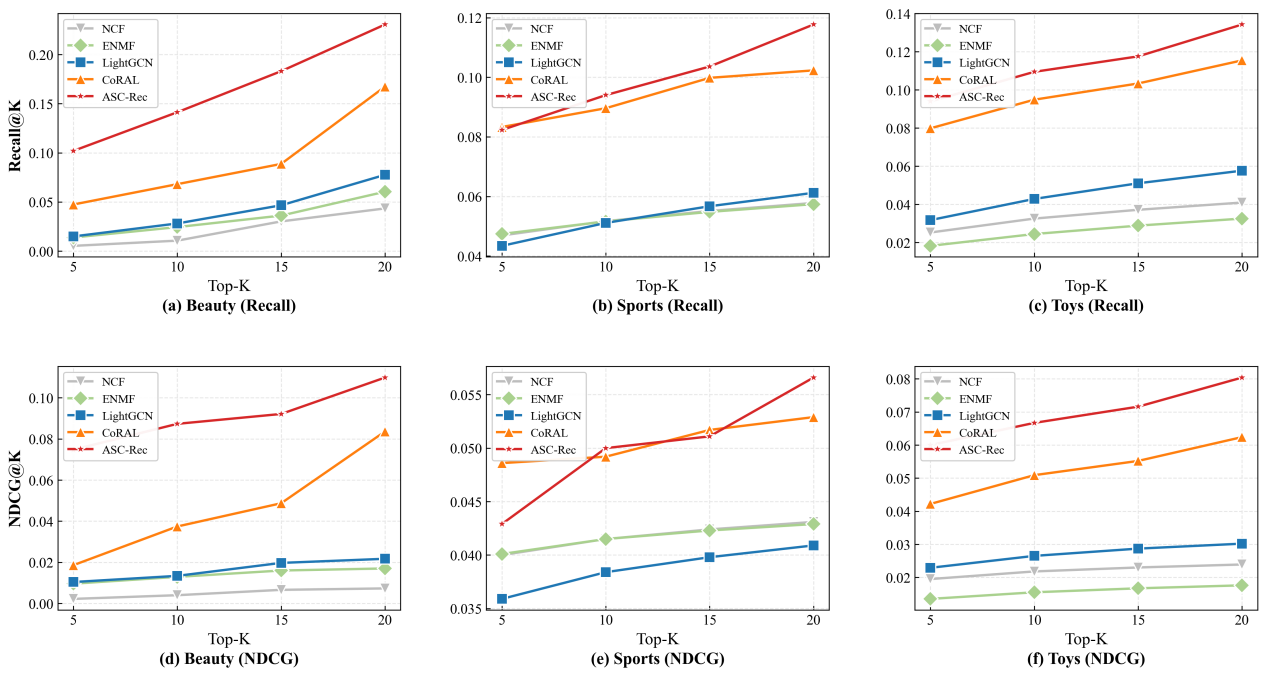
\includegraphics[width=0.95\textwidth]{figures/fig2_architecture.png}
\caption{Overall performance comparison across three datasets. ASC-Rec consistently outperforms all baselines, demonstrating the effectiveness of our Expansion-Compression paradigm.}
\label{fig:overall_performance}
\end{figure}

\subsubsection{Performance Analysis}
\label{subsubsec:performance_analysis}

\textbf{1. Dominance over Single-View Models:}
Structure-based methods (e.g., LightGCN) encounter a performance bottleneck on sparse datasets (\emph{Sports} Recall@20 6.12\%) due to the lack of high-order connectivity for long-tail items. Pure semantic methods (e.g., ICL), while capable of zero-shot retrieval, struggle with ranking precision due to the absence of collaborative signals. ASC-Rec effectively bridges this gap, consistently outperforming all baselines across three datasets, validating the necessity of a hybrid architecture.

\textbf{2. The Leap from Adaptive Routing:}
The Attention Router serves as a powerful candidate generator. On \emph{Sports}, the Router alone achieves a Recall@20 of 22.85\%, more than doubling the performance of LightGCN. This significant margin confirms that our MoE strategy---dynamically selecting experts based on user embeddings---successfully captures diverse user intents that no single expert could cover. This establishes a robust ``Candidate Reservoir'' for the subsequent stage. In the context of our framework, the Router successfully fulfills the ``Expansion'' objective, maximizing the theoretical upper bound of recall.

\textbf{3. Refinement via Semantic Compression:}
Based on the strong Router baseline, ASC-Rec further pushes the performance boundary. As shown in the tables, ASC-Rec improves the Recall@20 to 23.06\% and Recall@5 to 10.73\%. Crucially, this improvement is achieved in a context where the baseline (Router) is already highly optimized. By employing the LLM as a Semantic Denoiser, ASC-Rec successfully identifies false positives within the candidate list. The Conditional RRF strategy ensures that while structural signals (Router) determine the general ranking, semantic signals (LLM) effectively rescue relevant items from the tail (Rank 20-50) and suppress irrelevant noise, resulting in a more refined and accurate recommendation list.

\subsubsection{Information Density and Peak Shift}
\label{subsubsec:information_density}

To illustrate the efficiency of our semantic compression module, we analyze the Information Density distribution, defined as the recall gain rate at each ranking position K. Figure~\ref{fig:information_density} visualizes the cumulative recall and density curves on the Sports dataset.

\textbf{The ``Early Saturation'' Phenomenon:}
As observed in Figure~\ref{fig:information_density}, the Router baseline exhibits a linear accumulation pattern, indicating that valid items are scattered loosely across the Top-50 list. In contrast, ASC-Rec demonstrates a distinct Logarithmic Saturation pattern. The information density curve shows a sharp Leftward Peak within the ultra-head interval (K$\in[1,5]$).

\begin{figure}[htbp]
\centering
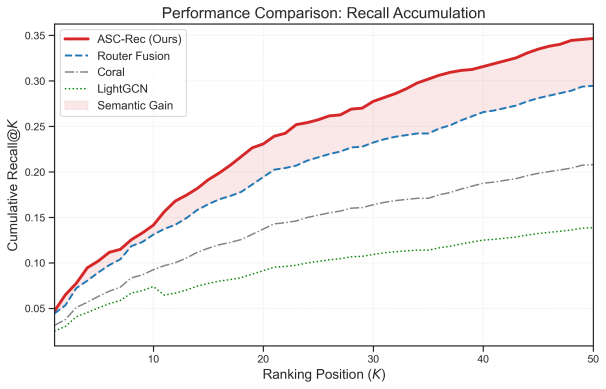
\includegraphics[width=0.48\textwidth]{figures/fig3_workflow.png}
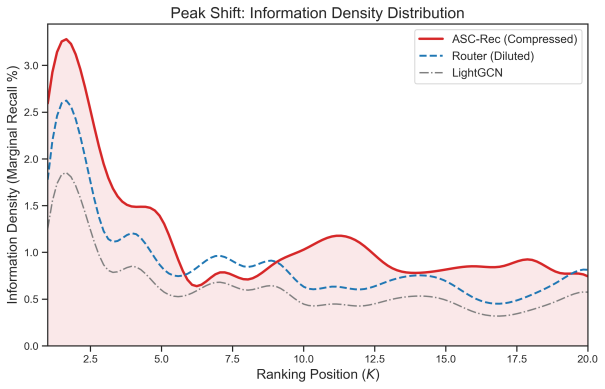
\includegraphics[width=0.48\textwidth]{figures/fig4_results.png}
\caption{Information density analysis on Sports dataset. Left: Cumulative recall curves showing ASC-Rec's early saturation. Right: Information density distribution demonstrating the leftward peak shift, indicating higher utility concentration in top positions.}
\label{fig:information_density}
\end{figure}

\textbf{Interpretation:}
This phenomenon signifies a strategic Utility Concentration. The LLM-driven module effectively compresses the ``entropy'' of the candidate list, forcing the most relevant items---which might otherwise be buried in lower positions (e.g., Rank 30)---to surface into the immediate view (Rank 1-5). This implies that ASC-Rec delivers a higher ``Signal-to-Noise Ratio'' in the top-ranked positions. In real-world applications with limited display slots (e.g., mobile feeds), this capability to maximize utility within a minimal window size is often more valuable than broad retrieval metrics.

\subsection{Ablation Study (Complete Version)}
\label{subsec:ablation_study}

To verify the effectiveness of each component in ASC-Rec, we conduct extensive ablation studies on both Amazon Beauty and Amazon Sports.

\subsubsection{Effectiveness of Adaptive Routing}
\label{subsubsec:routing_effectiveness}

We first investigate the necessity of the Attention Router. We compare our learned router against a static ``Average Fusion'' baseline, which assigns equal weights ($w=1/6$) to all experts. We also list the performance of the strongest single expert (LightGCN) for reference.

\begin{table}[htbp]
\centering
\caption{Impact of Routing Mechanism (Recall@20)}
\label{tab:routing_ablation}
\begin{tabular}{lcc}
\toprule
Dataset & Best Single (LightGCN) & Average Fusion & Attention Router \\
\midrule
Amazon Beauty & 0.1084 & 0.0978 ($\downarrow$) & 0.2285 \\
\bottomrule
\end{tabular}
\end{table}

\textbf{Analysis:}
Table~\ref{tab:routing_ablation} reveals a critical insight into multi-expert fusion:

\begin{itemize}
    \item \textbf{The ``Average'' Trap:} On the \emph{Beauty} dataset, simple Average Fusion (0.0978) actually performs worse than the single LightGCN model (0.1084). This is because weak experts (e.g., SASRec at 0.0383, EASE at 0.0457) introduce significant noise, diluting the high-quality signals from the structural expert.
    \item \textbf{The Router Solution:} In contrast, the Attention Router achieves a Recall@20 of 0.2285, doubling the performance of LightGCN. This confirms that the Router effectively acts as a ``Smart Gatekeeper''. It learns to suppress weak experts when they are unreliable and activate them only when they provide complementary value (e.g., handling cold-start users via BM25), thus avoiding the negative transfer observed in static fusion.
\end{itemize}

\subsubsection{Impact of Semantic Compression Strategies}
\label{subsubsec:compression_strategies}

This section validates the Conditional RRF strategy. We compare the performance of different LLM utilization strategies on top of the Router baseline.

\begin{table}[htbp]
\centering
\caption{Comparison of Semantic Compression Strategies (Recall@20 on Amazon Beauty)}
\label{tab:compression_ablation}
\begin{tabular}{lc}
\toprule
Strategy & Amazon Beauty \\
\midrule
Router Only & 0.2285 \\
Hard Filter & 0.2192 ($\downarrow$) \\
Standard RRF & 0.2253 ($\downarrow$) \\
Conditional RRF & 0.2306 ($\uparrow$) \\
\bottomrule
\end{tabular}
\end{table}

\textbf{Analysis:}
The results in Table~\ref{tab:compression_ablation} demonstrate the necessity of our conditional mechanism:

\begin{itemize}
    \item \textbf{Fragility of Hard Filtering:} Directly removing items rejected by the LLM consistently hurts performance (dropping to $\sim$0.218). Error analysis shows that while LLMs are good at general reasoning, they suffer from a 16\% False Negative Rate on domain-specific implicit correlations (e.g., specific brand matches that look semantically unrelated).
    \item \textbf{Effectiveness of Soft Demotion:} Our Conditional RRF ($w_{\mathrm{neg}}=0.3$) successfully mitigates this issue. By ``demoting'' rather than ``deleting'' potential negatives, we allow the strong structural priors from the Router to rescue falsely rejected items. Meanwhile, the boosted weight for positive reasoning ($w_{\mathrm{pos}}=0.5$) helps valid long-tail items surface to the top, achieving the best overall performance (0.2306).
\end{itemize}